\chapter{Longer downsampling rates for acoustic classification
\label{chap:9}}

During the study of tool wear classification via acoustic spectra, 
different preprocessing methods were tested. 
The fraction of dimensions that showed significant differences 
across wear categories was used to predict preprocessor performance.
For example, the time domain data does not generally have specific 
time offsets whose sample value correlates to the wear category.
In comparison, the frequency domain data at different frequencies
is likely to change between wear categories due to the changing tool geometry
and increased cutting forces that accompany tool wear.

The results of our study indicated that the unmodified Fourier spectra magnitude values
provided the better classification results than attempting to transform the values further.
For example, the square of these values, a.k.a. the power spectral density, 
was tested as well as the square root of the values.
Plots of data distributions for the wear categories before normalization are shown in \ref{fig:basis}.
Plots of the significant differences between wear categories for each type of preprocessing 
is shown in \ref{fig:basis_compare}. Normalization has no effect on the significance of the differences.

Other types of preprocessing tricks were applied in an effort 
to maximize the fraction of dimensions which correlate with tool wear.
Filtering in the frequency domain was applied to  smooth 
the frequency response over the sampled domain.
This way, bands of irrelevant frequencies can be brought closer to the
values of neighboring bands that are significant. 
Also, boost filters were applied to increase peaks that are
relevant to wear category and exaggerate the trends.
Ultimately, these techniques did not improve upon the performance
given by the unmodified Fourier spectra magnitude.

The result of low pass filtering in the frequency domain is similar
to the effect of downsampling followed by up-sampling 
via zero padding in the time domain. 
The variance of the 
frequency response over the frequency domain is reduced by clumping
the modes together.
Assuming vibrations are caused by a system that is 
stationary in the short term, the variance of the frequency 
response measurement is reduced by using a longer sample.
This provides increased frequency resolution over the domain,
but at the cost of longer response and classification times.

Window shapes can have subtle but important effects on results.
For the concrete sample in this work, much of the acoustic energy was
below 6 kHz. The higher frequencies still had significant differences,
but the environment in an underground mine dampens these frequencies while
being fairly permissive to lower frequencies. 
Our chosen window captures the lower frequencies, but other windows
could allow better performance from higher frequencies.
Future work should investigate optimal window shapes.

\begin{figure}[t]
\centering
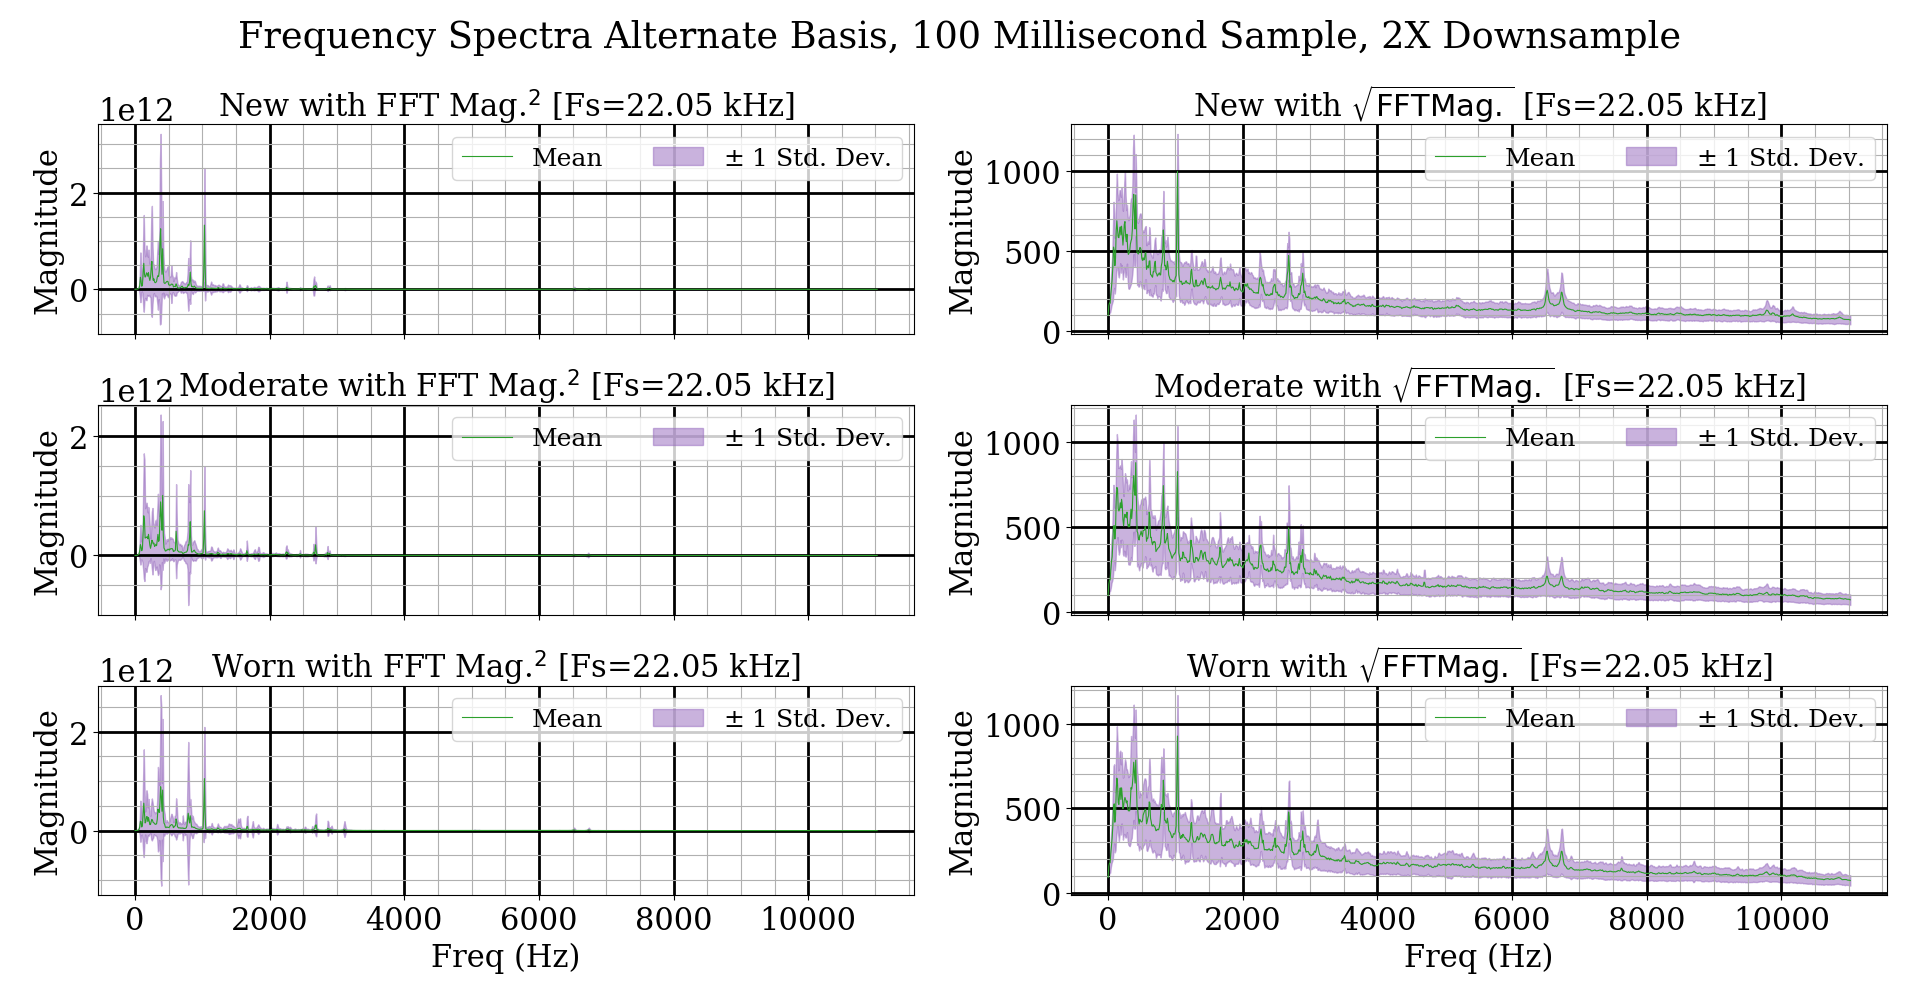
\includegraphics[width=0.85\textwidth]{ch_9_frequencies.png}
\caption{
Data distributions for the tested wear categories using additional Fourier based preprocessing techniques.
The square of the magnitude is an estimate of the power spectral density of the signal.
The square root of the magnitude conditions the signal so that the higher frequencies with small magnitudes
have magnitudes closer to the lower frequencies with large magnitudes.
Neither of these methods gave better classification results than the unmodified Fourier spectra magnitude.
}
\label{fig:basis}
\end{figure}

\begin{figure}[h]
\centering
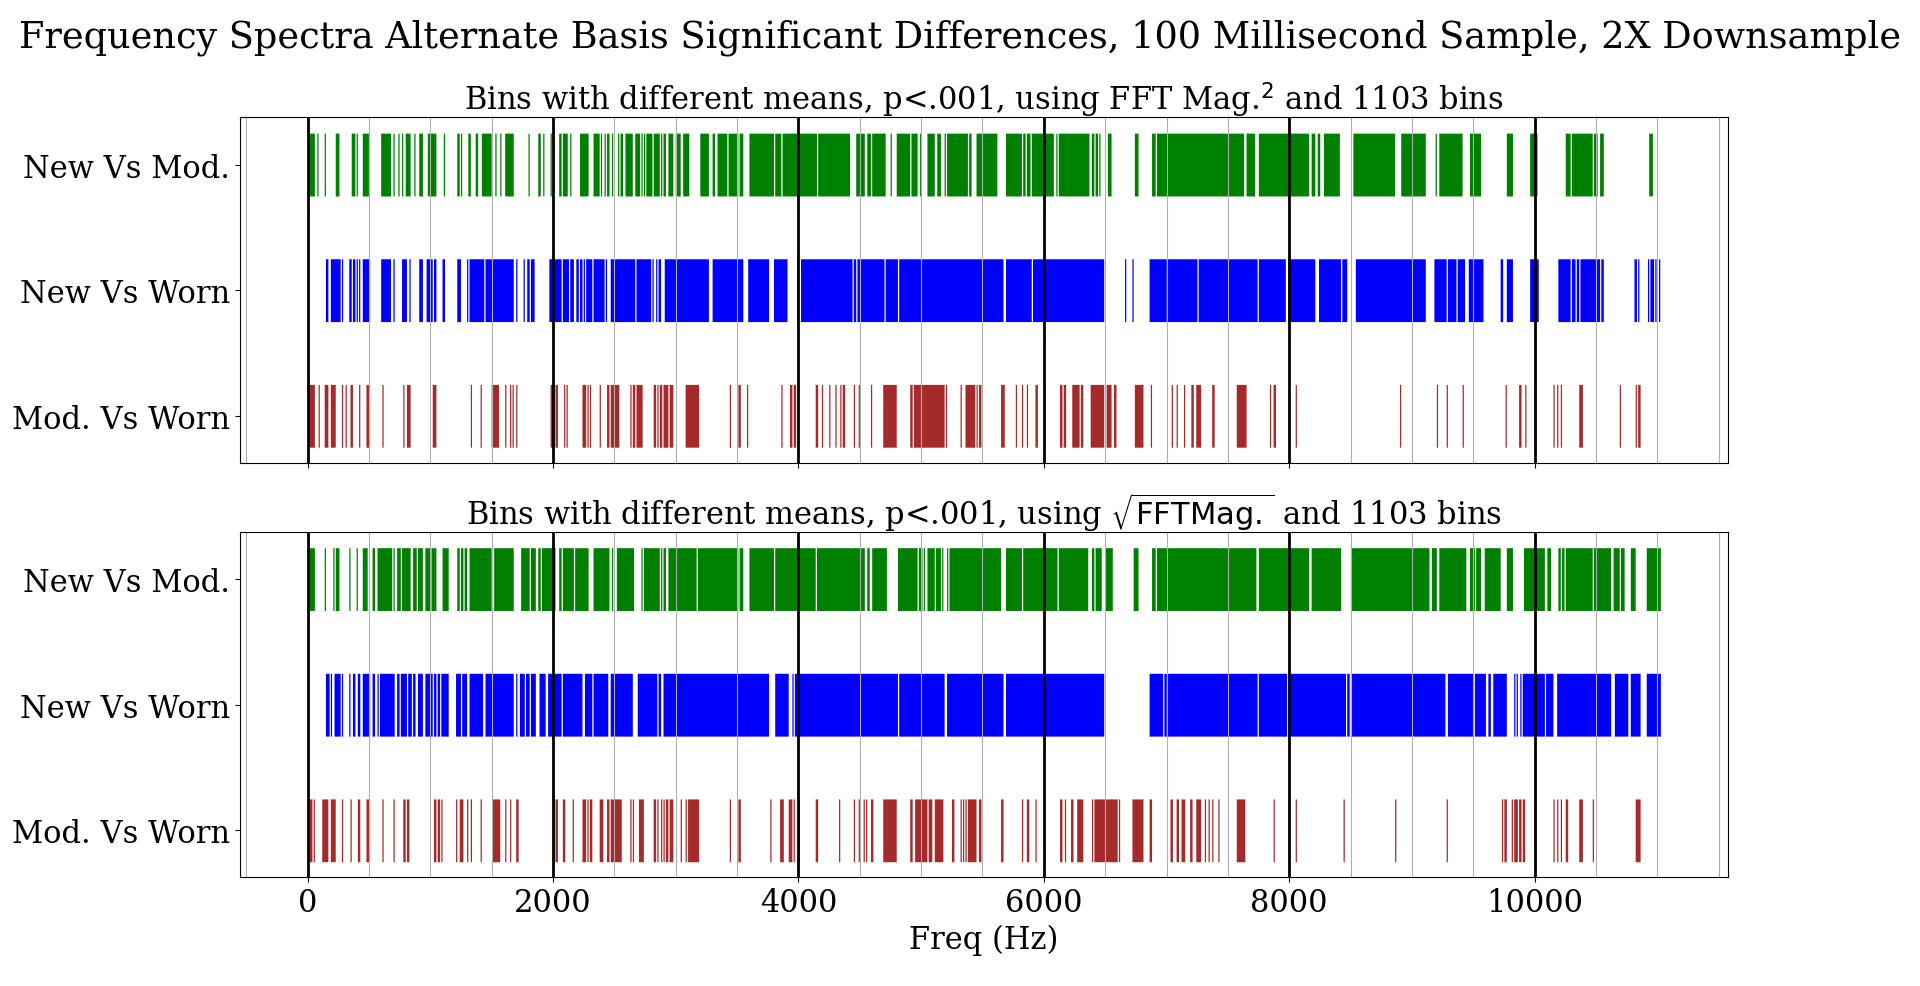
\includegraphics[width=0.85\textwidth]{ch_9_frequencies_compare.png}
\caption{
Tests for significant differences in frequency content between wear categories for the additional 
Fourier based preprocessing techniques. The square root was able to bring the differences between 
more high frequencies into significance compared to the square, or power spectral density. 
Squaring a signal will make outliers larger, while the square root conditions by bringing all numbers closer to unit value.
Neither of these methods adds more information or improves the signal basis for classification over the spectra magnitude. 
However, they do perform much better compared to using time domain data.
}
\label{fig:basis_compare}
\end{figure}

